%%%%%%%%%%%%%%%%%%%%%%%%%%%%%%%%%%%%%%%%%%%%%%%%%%%%%%%%%%%%%%%%
%%                                                            %%
%%   essentialsOfLatin, Italian translation 2017              %%
%%                                                            %%
%% From:  Henry C. Pearson, Essentials Of Latin For Beginners %%
%%        (1915, New York, American Book Company)             %%
%%                                                            %%
%%    https://archive.org/details/essentialslatin04peargoog   %%
%%                                                            %%
%% Translated by g.p.ciceri <gp.ciceri@gmail.com>             %%
%% ---------------------------------------------------------- %%
%% This translation is Licensed under                         %%
%% Creative Commons Attribution-ShareAlike 4.0 International  %%
%% https://creativecommons.org/licenses/by-sa/4.0/            %%
%%                                                            %%
%%%%%%%%%%%%%%%%%%%%%%%%%%%%%%%%%%%%%%%%%%%%%%%%%%%%%%%%%%%%%%%%

% āēīōū
% ăĕĭŏŭ




\documentclass[nols]{tufte-handout}

%\geometry{showframe} % display margins for debugging page layout

\usepackage{fontspec}
\usepackage{ifxetex}
\setmainfont[Path=./fonts/palatino-linotype/, ItalicFont=palai.ttf, BoldFont=palab.ttf]{pala.ttf}


% \defaultfontfeatures{Mapping=tex-text}
% \setromanfont[Path=./fonts/TeX-Gyre-Schola/,Mapping=tex-text]{TeX Gyre Schola}
% \setsansfont[Path=./fonts/TeX-Gyre-Heros/,Scale=MatchLowercase,Mapping=tex-text]{TeX Gyre Heros}
% \setmonofont[Path=./fonts/TeX-Gyre-Cursor/,Scale=MatchLowercase]{TeX Gyre Cursor}

\usepackage{lipsum}
\usepackage{url}
\usepackage{longtable}
\usepackage{stackengine}

\usepackage{graphicx} % allow embedded images
  \setkeys{Gin}{width=\linewidth,totalheight=\textheight,keepaspectratio}
  \graphicspath{{graphics/}} % set of paths to search for images
\usepackage{amsmath}  % extended mathematics
\usepackage{booktabs} % book-quality tables
\usepackage{units}    % non-stacked fractions and better unit spacing
\usepackage{multicol} % multiple column layout facilities
\usepackage{lipsum}   % filler text
\usepackage{fancyvrb} % extended verbatim environments
  \fvset{fontsize=\normalsize}% default font size for fancy-verbatim environments

% Standardize command font styles and environments
\newcommand{\doccmd}[1]{\texttt{\textbackslash#1}}% command name -- adds backslash automatically
\newcommand{\docopt}[1]{\ensuremath{\langle}\textrm{\textit{#1}}\ensuremath{\rangle}}% optional command argument
\newcommand{\docarg}[1]{\textrm{\textit{#1}}}% (required) command argument
\newcommand{\docenv}[1]{\textsf{#1}}% environment name
\newcommand{\docpkg}[1]{\texttt{#1}}% package name
\newcommand{\doccls}[1]{\texttt{#1}}% document class name
\newcommand{\docclsopt}[1]{\texttt{#1}}% document class option name
\newenvironment{docspec}{\begin{quote}\noindent}{\end{quote}}% command specification environment

% concetti morfosintattici
\usepackage{xspace} 
\newcommand{\noun}{\textsc{sostantivo}\xspace}
\newcommand{\nouns}{\textsc{sostantivi}\xspace}
\newcommand{\adject}{\textsc{aggettivo}\xspace}
\newcommand{\adjects}{\textsc{aggettivi}\xspace}
\newcommand{\gnumber}{\textsc{numero}\xspace}
\newcommand{\gnumbers}{\textsc{numeri}\xspace}
\newcommand{\gender}{\textsc{genere}\xspace}
\newcommand{\genders}{\textsc{generi}\xspace}
\newcommand{\gcase}{\textsc{caso}\xspace}
\newcommand{\gcases}{\textsc{casi}\xspace}
\newcommand{\tense}{\textsc{tempo}\xspace}
\newcommand{\mood}{\textsc{modo}\xspace}
\newcommand{\gverb}{\textsc{verbo}\xspace}
\newcommand{\gverbs}{\textsc{verbi}\xspace}
\newcommand{\adjective}{\textsc{aggettivo}\xspace}
\newcommand{\nom}{\textsc{nom}\xspace}
\newcommand{\gen}{\textsc{gen}\xspace}
\newcommand{\dat}{\textsc{dat}\xspace}
\newcommand{\acc}{\textsc{acc}\xspace}
\newcommand{\voc}{\textsc{voc}\xspace}
\newcommand{\abl}{\textsc{abl}\xspace}
\newcommand{\gexit}{\textsc{uscita}\xspace}
\newcommand{\gexits}{\textsc{uscite}\xspace}
\newcommand{\declinazione}{\textsc{declinazione}\xspace}
\newcommand{\masc}{\textsc{maschile}\xspace}
\newcommand{\femm}{\textsc{femminile}\xspace}
\newcommand{\neut}{\textsc{neutro}\xspace}

\newcommand{\indic}{\textsc{indicativo}\xspace}
\newcommand{\imper}{\textsc{imperativo}\xspace}
\newcommand{\gcong}{\textsc{congiuntivo}\xspace}
\newcommand{\ott}{\textsc{ottativo}\xspace}
\newcommand{\partic}{\textsc{participio}\xspace}
\newcommand{\infin}{\textsc{infinito}\xspace}

\newcommand{\pres}{\textsc{presente}\xspace}
\newcommand{\imperf}{\textsc{imperfetto}\xspace}
\newcommand{\aor}{\textsc{aoristo}\xspace}
\newcommand{\fut}{\textsc{futuro}\xspace}
\newcommand{\perf}{\textsc{perfetto}\xspace}
\newcommand{\pperf}{\textsc{piuccheperfetto}\xspace}

\newcommand{\sing}{\textsc{singolare}\xspace}
\newcommand{\plur}{\textsc{plurale}\xspace}
\newcommand{\dual}{\textsc{duale}\xspace}

\newcommand{\si}{\textsc{sing}\xspace}
\newcommand{\pl}{\textsc{plur}\xspace}
\newcommand{\du}{\textsc{dual}\xspace}

\newcommand{\att}{\textsc{attivo}\xspace}
\newcommand{\med}{\textsc{medio}\xspace}
\newcommand{\pass}{\textsc{passivo}\xspace}
\newcommand{\medpass}{\textsc{medio-passivo}\xspace}


% italianitudini
\renewcommand{\figurename}{Figura}
\renewcommand{\tablename}{Tabella}
\renewcommand{\contentsname}{Indice}

% fix per un qualche problema
\ifxetex
  \newcommand{\textls}[2][5]{%
    \begingroup\addfontfeatures{LetterSpace=#1}#2\endgroup
  }
  \renewcommand{\allcapsspacing}[1]{\textls[15]{#1}}
  \renewcommand{\smallcapsspacing}[1]{\textls[10]{#1}}
  \renewcommand{\allcaps}[1]{\textls[15]{\MakeTextUppercase{#1}}}
  \renewcommand{\smallcaps}[1]{\smallcapsspacing{\scshape\MakeTextLowercase{#1}}}
  \renewcommand{\textsc}[1]{\smallcapsspacing{\textsmallcaps{#1}}}
\fi

% too many float...
\extrafloats{100}

\title{Essentials Of Latin. Elementi di Latino. \newline Lezione XXIII - Aggettivi della Seconda Classe a Tre Uscite. Ablativo di Limitazione.}

\author[gpciceri]{a cura di Milagathòs: Milo's help to enjoy humanities.}

\date{25 Febbrajo 2017} % without \date command, current date is supplied


\begin{document}

\hyphenation{co-niu-ga-zio-ne}

\maketitle% this prints the handout title, author, and date

\begin{marginfigure}[-2.5cm]
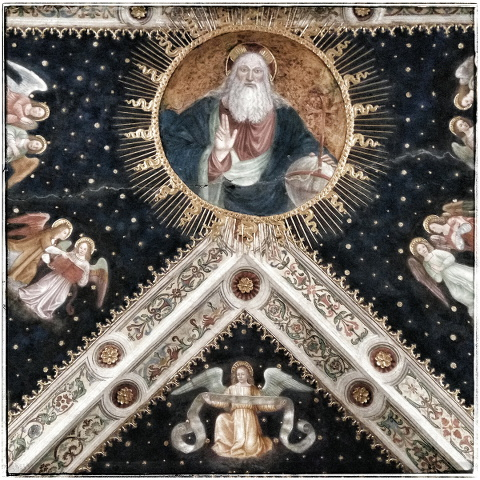
\includegraphics{smallthumb-lesson_XI.jpeg}
\setfloatalignment{b}
\end{marginfigure}


\begin{abstract}
\noindent
Queste lezioni riprendono il testo introduttivo al Latino di Pearson\cite{pearson1915}, del quale seguono la numerazione; la struttura di ogni lezione è piuttosto regolare: inizia con \textsc{cenni di morfologia e di sintassi latina}, seguita da un \textsc{piccolo vocabolario} per il lessico; ci sono infine vari \textsc{esercizi} di traduzione e di composizione latina.

\bigskip
\noindent
Lezione XXIII - Aggettivi della Seconda Classe a Tre Uscite. Ablativo di Limitazione. Vocabolario, esercizi.
\end{abstract}

%\printclassoptions

\newthought{155.} Gli aggettivi della Seconda Classe (corrispondenti ai nomi della Terza Declinazione) si dividono in tre gruppi, a seconda che al nominativo singolare presentino, rispettivamente, tre, due e una sola terminazione.

% āēīōū
% ăĕĭŏŭ


\begin{fullwidth}
\begin{table}[!htbp]
  \centering
  \begin{tabular}{l l l l}
    %\toprule
	\multicolumn{4}{c}{\textbf{ācer}, \textit{acuto, aspro, fiero}} \\
	\multicolumn{4}{c}{\textsc{Tema} \textbf{ācri-}, \textsc{Radice} \textbf{ācr-}} \\
	
	\multicolumn{4}{c}{\textsc{Singolare}} \\
	& \multicolumn{1}{c}{\textsc{Maschile}} & \multicolumn{1}{c}{\textsc{Femminile}} & \multicolumn{1}{c}{\textsc{Neutro}} \\
	
    \textsc{Nom.} & ācer & ācr\textbf{is} & ācr\textbf{e} \\
    \textsc{Gen.} & ācr\textbf{is} & ācr\textbf{is} & ācr\textbf{is} \\
    \textsc{Dat.} & ācr\textbf{i} & ācr\textbf{i} & ācr\textbf{i} \\
    \textsc{Acc.} & ācr\textbf{em} & ācr\textbf{em} & ācr\textbf{e} \\
    \textsc{Voc.} & ācer & ācr\textbf{is} & ācr\textbf{e} \\
    \textsc{Abl.} & ācr\textbf{i} & ācr\textbf{i} & ācr\textbf{i} \\
	
	\multicolumn{4}{c}{\textsc{Plurale}} \\
	
    \textsc{Nom.} & ācr\textbf{es} & ācr\textbf{es} & ācr\textbf{ia} \\
    \textsc{Gen.} & ācr\textbf{ium} & ācr\textbf{ium} & ācr\textbf{ium} \\
    \textsc{Dat.} & ācr\textbf{ibus} & ācr\textbf{ibus} & ācr\textbf{ibus} \\
    \textsc{Acc.} & ācr\textbf{es} & ācr\textbf{es} & ācr\textbf{ia} \\
    \textsc{Voc.} & ācr\textbf{es} & ācr\textbf{es} & ācr\textbf{ia} \\
    \textsc{Abl.} & ācr\textbf{ibus} & ācr\textbf{ibus} & ācr\textbf{ibus} \\
	
    %\bottomrule
  \end{tabular}
  %\caption{}
  \label{tab:normaltab}
  %\zsavepos{pos:normaltab}
\end{table}
\end{fullwidth}


\newthought{Osservazioni}
\begin{itemize}
\item[\textsc{1.}] Gli aggettivi della seconda classe hanno i temi in -i-, l'ablativo singolare esce in -i.  
\end{itemize}

\newthought{156. Frasi Modello.} Esamina le seguenti frasi:
\begin{itemize}
\item[\textsc{1.}] \textbf{Helvetii Gallos virtute superant}, \textit{Gli Elvezi superan i Galli in valore}.  
\item[\textsc{2.}] \textbf{Vir nomine, non factis, amicus erat}, \textit{l'uomo era amico di nome, non nei fatti}.  
\end{itemize}

Gli ablativi \textbf{virtute, nomine, factis} indicano \textit{in che cosa, rispetto a cosa} si afferma il significato del verbo o del nome; la prima frase dice che gli Elvezi sono superiori ai Galli rispetto al \textit{valore militare}, non in dimensioni, velocità o ad altro. 

\newthought{157. Regola \textemdash Ablativo di Limitazione (di Specificazione).} L'ablativo di Limitazione (o di Specificazione) indica rispetto a cosa, in che senso, limitatamente a cosa vada inteso il significato del verbo, del nome o dell'aggettivo cui questo ablativo si riferisce. Non c'è bisogno di alcuna preposizione.

% āēīōū
% ăĕĭŏŭ

\newthought{158. Vocabolario}

\begin{multicols}{2}
    \noindent \hangindent=1em \textbf{altus, -a, -um}, agg., \textit{alto, profondo}.  \\
	\noindent \hangindent=1em \textbf{angustus, -a, -um}, agg., \textit{stretto, piccolo}.  \\
	\noindent \hangindent=1em \textbf{noster, nostra, nostrum}, agg., \textit{nostro}.  \\
	\noindent \hangindent=1em \textbf{acer, acris, acre}, agg., \textit{acuto, fiero, aspro}.  \\
	\noindent \hangindent=1em \textbf{equester, equestris, equestre}, agg., \textit{della cavalleria, equestre}.  \\
	\noindent \hangindent=1em \textbf{finis, finis}, m., \textit{fine}, al pl. , \textit{confine}.  \\
    \noindent \hangindent=1em \textbf{finitimus, -a, -um}, agg., \textit{confinante, vicino}.  \\
    \noindent \hangindent=1em \textbf{finitimi, -orum}, m., \textit{confinanti, vicini}.  \\
	
	\noindent \hangindent=1em \textbf{quod}, cong., \textit{perché, poiché}.  \\
	\noindent \hangindent=1em \textbf{-que}, cong., \textit{e}, enclitica, sempre attaccata alla seconda delle due parole collegate.  \\
	
    \noindent \hangindent=1em \textbf{magnitudo, magnitudinis}, f., \textit{grandezza}.  \\
	
    
\end{multicols}


\newthought{159. Esercizi di Ripasso}
\\
\textsc{I.} \quad
\textsc{1.}~Dux filium propter virtutem laudaverat. \quad
\textsc{2.}~Pax quattuor mensibus a Caesare cum multis civitatibus erat confirmata. \quad
\textsc{3.}~Multa nocte copiae ex agris in castra convocabantur. \quad
\textsc{4.}~Milites hieme in hiberna convocati sunt. \quad
\textsc{5.}~Multi incolae gladiis equitum vulnerati erant.
\\
\textsc{II.} \quad
\textsc{1.}~Perché i Galli si sollevarono? \quad
\textsc{2.}~La città era stata presa a Marzo. \quad
\textsc{3.}~All'alba, il generale diede del cibo ai suoi soldati. \quad
\textsc{4.}~Il console soffrì per la mancanza della cavalleria.

\newthought{160. Esercizi}
\\
\textsc{I.} \quad
\textsc{1.}~Castra Caesaris in Helvetiorum finibus erant. \quad
\textsc{2.}~Iter per fines nostros angustum erat. \quad
\textsc{3.}~Romani virtute, non magnitudine corporis, Gallos superabant. \quad
\textsc{4.}~Equestres copiae hostium magna cum virtute pugnaverant. \quad
\textsc{5.}~Flumina Galliae angusta et alta erant. \quad
\textsc{6.}~Equites a Caesare laudati sunt, quod hostes celeritate superaverunt. \quad
\textsc{7.}~Acres peritaeque erant copiae consulis. \quad
\textsc{8.}~Pedites Caesaris proelio acres erant. \quad
\textsc{9.}~Cur Helvetii a ducibus incitati sunt? Quod altis montibus et fluminibus latis continebantur. \quad
\textsc{10.}~Hostes equestri proelio superati erant.
\\
\textsc{II.} \quad
\textsc{1.}~La battaglia con la nostra cavalleria fu aspra. \quad
\textsc{2.}~Avete visto molti fiumi profondi? \quad
\textsc{3.}~Superiamo i nostri vicini nel valore della cavalleria. \quad
\textsc{4.}~C'è una strada stretta attraverso i territori dei nostri vicini. \quad
\textsc{5.}~Il generale fu ferito al piede. \quad
\textsc{6.}~Gli Elvezi presero molte città perché combattevano con grande coraggio.

\begin{figure}[!b]
  %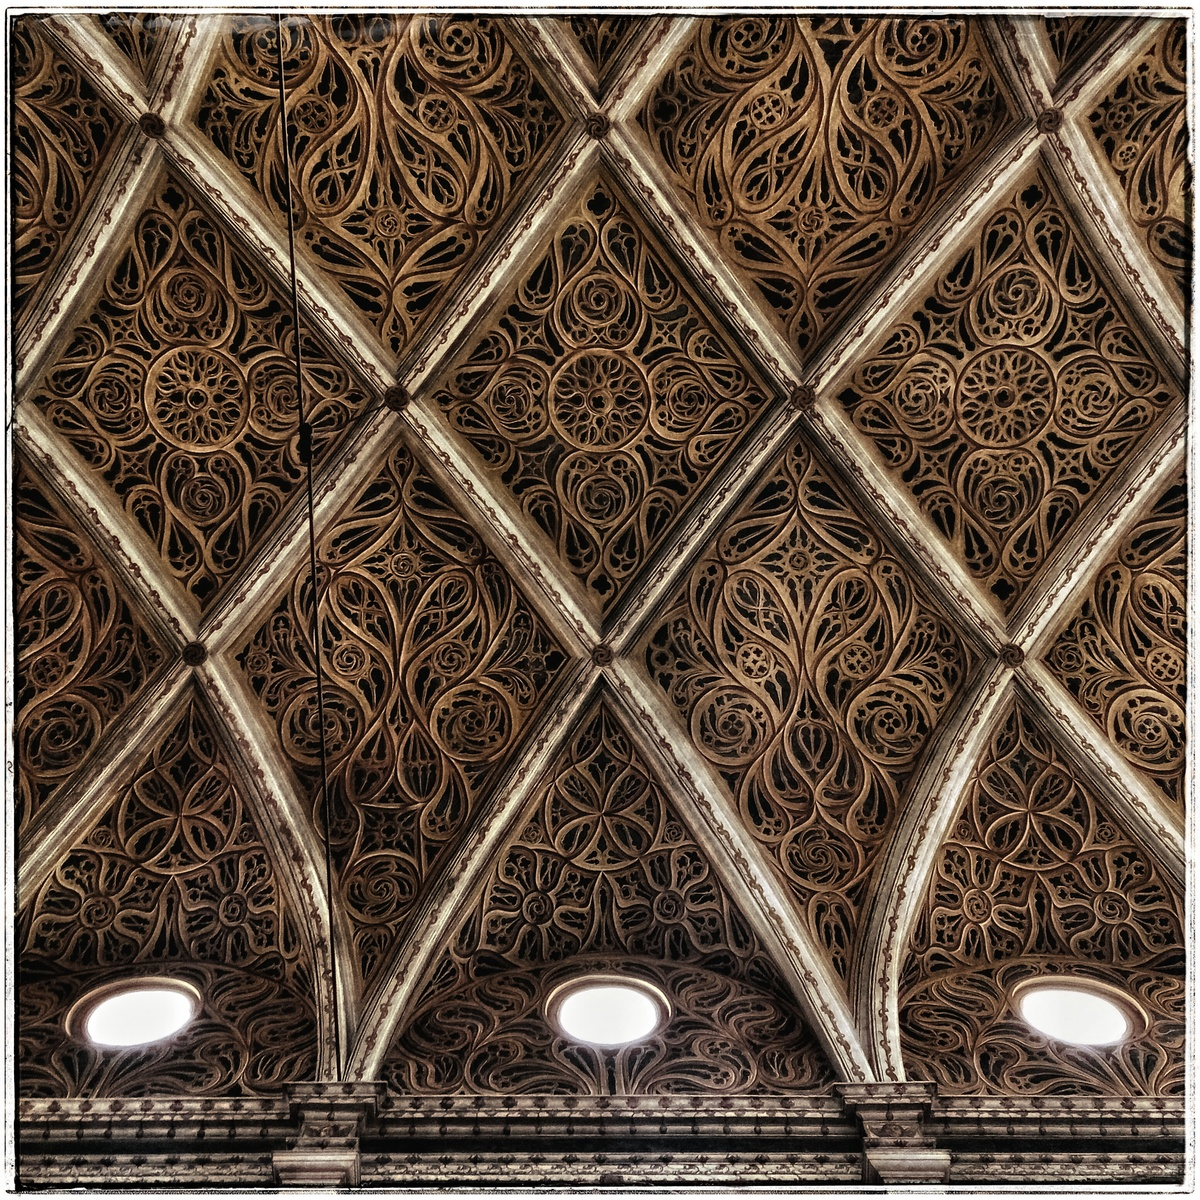
\includegraphics{thumb-lesson_XXI.jpeg}
  %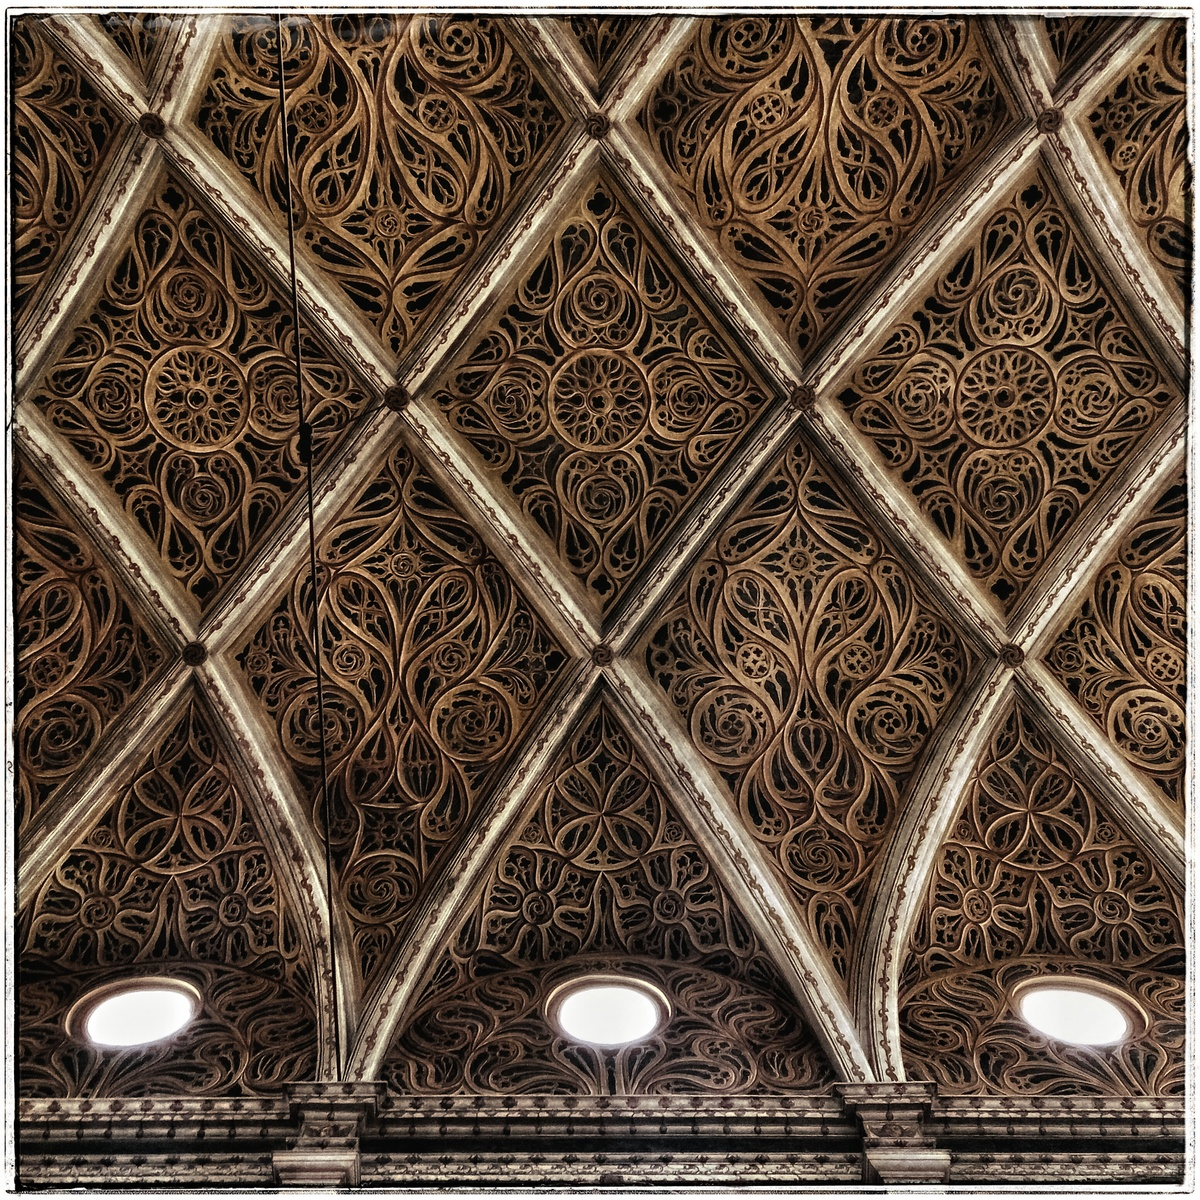
\includegraphics[width=0.9\linewidth]{thumb-lesson_XXI.jpeg}
  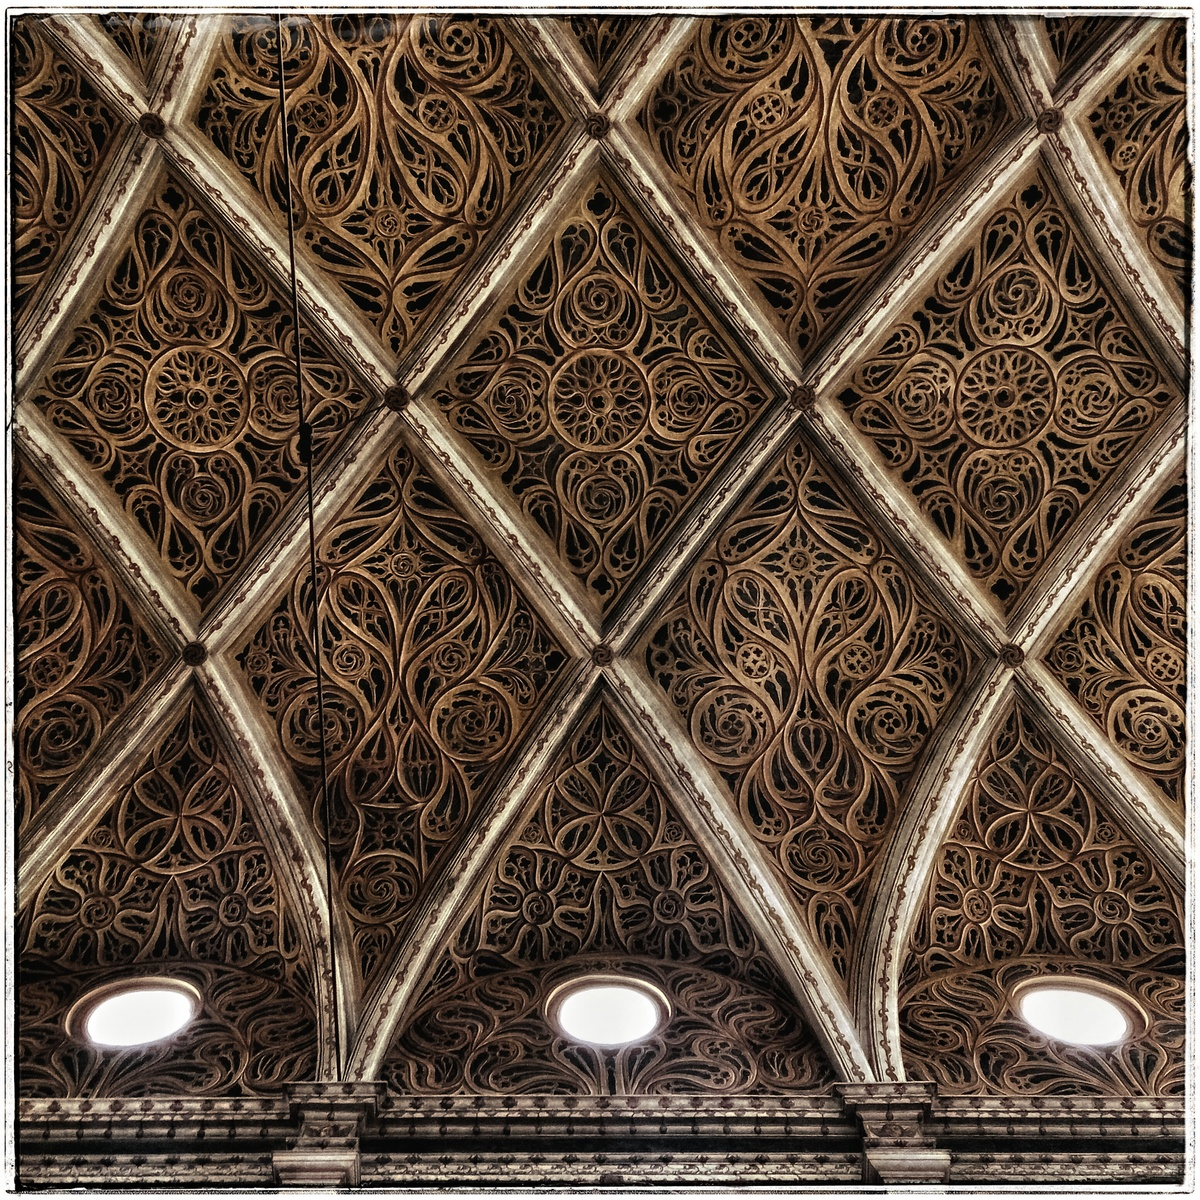
\includegraphics{thumb-lesson_XXI.jpeg}
  \caption{Milano: San Maurizio al Monastero Maggiore}
  \label{fig:textfig}
  %\zsavepos{pos:textfig}
  %\setfloatalignment{b}
\end{figure}

 

\nobibliography{latinBiblio}
\bibliographystyle{alpha}


\end{document}
